\PassOptionsToPackage{hyperfootnotes=false}{hyperref}
\documentclass{beamer}
\usefonttheme{professionalfonts}
%\usetheme{Rochester}
%\usetheme{AnnArbor}
\usetheme{Szeged}
\useoutertheme{infolines}
\usecolortheme{dolphin}
\usepackage{graphicx}
\usepackage{booktabs}
% \usepackage[english]{babel}
\usepackage{multicol}
\usepackage{color}
\usepackage{xcolor}
%\usepackage{smartdiagram}


%\definecolor{carmine}{rgb}{0.59, 0.0, 0.09}
\usepackage{amsmath} 

\usepackage{graphicx}
\usepackage{tikz}
\usetikzlibrary{shapes.callouts}
\usepackage{multirow}

\usepackage[utf8]{inputenc}

\usepackage{enumerate}
\usepackage[shortlabels]{enumitem}
\usepackage{amsmath,amsthm,amssymb,amsfonts,mathrsfs,latexsym,stmaryrd}
\usepackage{tcolorbox}

\usepackage{color} 
\usepackage{amssymb, amsmath, amsbsy}
\usepackage{adjustbox,lipsum}
\usepackage{placeins}

\usepackage{textpos}
\usepackage{wrapfig}
\usepackage[spanish, es-tabla]{babel}

\usepackage{caption}
\setlength{\parindent}{0pt}

\usepackage{url}
\usepackage{float}
\usepackage{tikz}
\usetikzlibrary{patterns}


\title[ICS-162]{Econometría ICS-294\\ \small{Clase 21: Series de tiempo}}

\author{Pedro Comte Hidalgo}
\institute[USM]
{Universidad Técnica Federico Santa María\\ % Your institution for the title page
	\medskip
	\textit{} % Your email address
	
}
\logo{

\includegraphics[width=1cm]{Logo.png}
}
\date{}
\newcommand\Fontvi{\fontsize{9}{7.2}\selectfont}
\begin{document}


\frame{\titlepage}




% \begin{frame}
% \frametitle{Test de Breusch-Godfrey para correlación serial  de orden (1) {\bf del error}}

% \begin{itemize}
%   \item Para series de tiempo existen varios test.
%   \item Con la idea de una autocorrelación de orden 1:
%   \[
%   y_t = x_t \beta + \epsilon_t
%   \]
%   \[
%   \epsilon_t = \rho_1 \epsilon_{t-1}+v_t
%   \]
%   \item Test LM para testear \( H_0: \rho_1 = 0 \) (si hay un solo rezago, también se puede hacer test t).
%   \item Bajo \( H_0 \) cierta (no hay autocorrelación de orden 1) tenemos:
%  % \begin{itemize}
%     % \item Si \( \text{LM}_{\text{empírico}} > \chi^2_{\text{tabla}} \) \(\rightarrow\) ¡Rechazo \( H_0 \)!
%   %\end{itemize}
% \end{itemize}

% \end{frame}
% \begin{frame}
% \frametitle{Pasos Breusch-Godfrey}

% \begin{itemize}
%   \item La prueba de hipótesis la escribimos:
%   \[
%   H_0 : \rho_1 = 0
%   \]
%   \[
%   H_1 : \rho_1 \neq 0
%   \]
%   \item Pasos a seguir:
%   \begin{enumerate}
%     \item Estimar el modelo original por MCO y obtener los residuos \(\hat{\epsilon}\).
%     \item Estimar una regresión auxiliar de \(\hat{\epsilon}_t\) sobre el rezago: \(\hat{\epsilon}_t = \rho_0 + \rho_1 \hat{\epsilon}_{t-1}+ \nu_t\) .
%     \item Quedarse con el \(R^2\) y construir el estadístico LM de prueba:
%     \[
%     \text{LM} = nR^2_\epsilon
%     \]
%     \item Se compara con una \(\chi^2_p\) donde \(p\) es el número de rezagos (1 en este caso).
%     \item Si \(\text{LM} > \chi^2_p\) al \(\alpha \%\) \(\rightarrow\) rechazo la hipótesis nula de ausencia de autocorrelación. ¡Tenemos problema!
%   \end{enumerate}
% \end{itemize}

% \end{frame}


\begin{frame}
\frametitle{Caminata aleatoria (random walk)}

\begin{itemize}
  \item Muchas veces, las variables del modelo tienen persistencia: $ y_t = \rho y_{t-1} + \epsilon_t $.
  \item Si \(\rho = 1\), es una \textbf{caminata aleatoria}:
  \begin{itemize}
    \item Tiene una raíz unitaria o que es \textbf{integrada de orden 1.}
    \item Es un proceso no estacionario.
    %   \item Al igual que la tendencia 'determinística' que vimos antes, cuando tenemos una variable que se comporta de esta manera, vamos a tener que ajustarlo. Pero no va a alcanzar con agregar tendencia en este caso.
  \end{itemize}
  \item Cuando \(|\rho| < 1\)
  \begin{itemize}
    \item El proceso es estacionario.
    \item En este caso, podemos usar MCO sin inconveniente.
  \end{itemize}
\end{itemize}

\end{frame}

% \begin{frame}{Correlograma caminata aleatoria }


%     \begin{figure}
%         \centering
%         
\includegraphics[width=0.85\linewidth]{sem14//images/correlograma2.png}
%     \end{figure}
% \end{frame}


 \begin{frame}
\frametitle{Caminata aleatoria}

\begin{itemize}
  \item Si las series consideradas en una regresión  \(\rho = 1\), usar estas variables va a introducir correlación espuria entre las series.
  %\item Los datos tienen una tendencia en el tiempo, pero no es determinística (crece de forma constante) sino que es estocástica (crece pero de forma variante).
  \item Lo vamos a solucionar tomando la primera diferencia de la serie problemática:
  $
  \Delta y_t = y_t - y_{t-1} = \epsilon_t 
  $ y se trabaja con la diferencia y no el nivel.

\end{itemize} 
\end{frame}
\begin{frame}
\frametitle{Exploración gráfica - I(1)}

\begin{itemize}
  \item AR(1) con \(\rho = 1\)

             \begin{figure}
        \centering
        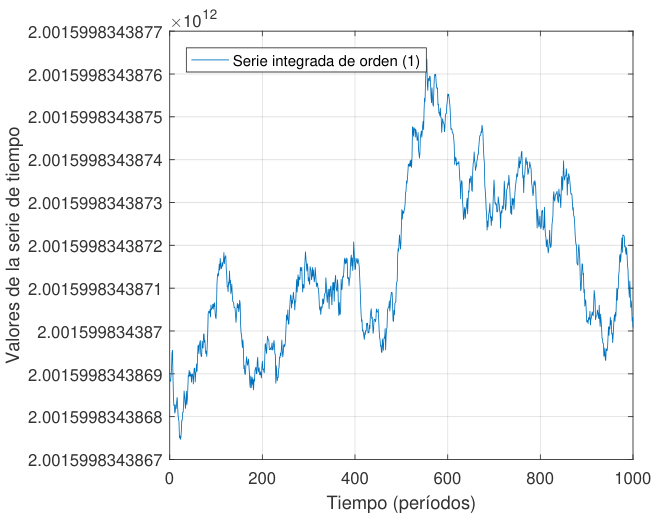
\includegraphics[width=0.7\linewidth]{images/ar1.png}
    \end{figure}


  \item La persistencia es muy alta.
\end{itemize}

\end{frame}


\begin{frame}{Caminata aleatoria }

\begin{itemize}
    \item En algunos casos, al graficar un proceso integrado puede parecer que presenta una tendencia. Sin embargo, esto se debe a la alta persistencia de la serie.

    \item Algunos autores han descrito tales tendencias como \textit{tendencias estocásticas} (véase Box, Jenkins y Reinsel, 1994), aunque no existe una definición generalmente aceptada de lo que constituye una tendencia estocástica.
\end{itemize}

    
\end{frame}

\begin{frame}
\frametitle{Exploración gráfica - Primera diferencia de una I(1)}

\begin{itemize}
  \item La serie con orden de integración 1 la diferenciamos, y ¿qué obtenemos?

             \begin{figure}
        \centering
        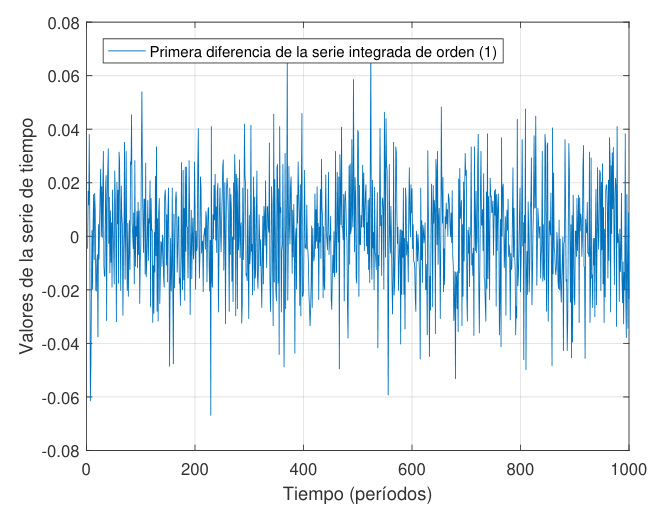
\includegraphics[width=0.7\linewidth]{images/i1.png}
    \end{figure}
  
  \item Muchas series macroeconómicas siguen este tipo de procesos.
\end{itemize}

\end{frame}


\begin{frame}
\frametitle{Inclusión de tendencias en los modelos de series temporales}

\begin{itemize}
  \item La "tendencia" de las series es como una variable omitida!
  \item Una manera de solucionar esto es incluir en el modelo una variable que recoja el crecimiento temporal: la tendencia.
  \item Una tendencia lineal \( t \) es una variable que crecerá una unidad cada año, lo más común empezando en 1.
\begin{center}
\begin{tabular}{c c}
\toprule
Año & t \\
\midrule
1940 & 1 \\
1941 & 2 \\
1942 & 3 \\
\vdots & \vdots \\
1960 & 20 \\
\bottomrule
\end{tabular}
\end{center}
  \item Se pueden ajustar tendencias cuadráticas (\( t^2 \)), o si la variable dependiente está en logs, la tendencia lineal será interpretada como tendencia exponencial.
\end{itemize}

\end{frame}


\begin{frame}
\frametitle{Inclusión de tendencias en los modelos de series temporales}

\begin{itemize}
  \item Cuando incluimos una tendencia determinística, el modelo que estimaremos será:
  \[
  y_t = \alpha_0 + \alpha_1 x_t + \alpha_2 t + \epsilon_t
  \]
  \item \(\alpha_2\) nos dice cuánto varía anualmente \( y_t \):
  \begin{itemize}
    \item \(\alpha_2 > 0\) y significativo: tendencia creciente.
    \item \(\alpha_2 < 0\) y significativo: tendencia decreciente.
  \end{itemize}
  \item La tendencia es predecible, determinada por el tiempo.

  \item \(\alpha_1\) nos dirá cuál es la relación entre \( x_t \) y \( y_t \) cuando les “quitamos” la tendencia.
\end{itemize}

\end{frame}




\begin{frame}{Raíces unitarias, tendencia estocástica y regresión espuria}
    \begin{itemize}
        \item Queremos estimar el modelo:
        \[
        Y_t = \beta_0 + \beta_1 X_t + u_t
        \]
        \item Supongamos que el proceso de cada variable es el siguiente:
        \[
        Y_t = \alpha_1 + \rho_1 Y_{t-1} + \epsilon_t
        \]
        \[
        X_t = \alpha_2 + \rho_2 X_{t-1} + v_t
        \]
        \item Si $-1 < \rho_i < 1$, entonces los procesos son AR(1) estacionarios y se puede hacer la regresión sin problema. 
        \item Si $\rho_i = 1$ la serie es una caminata aleatoria. 
     Esto hace que se encuentren relaciones espurias entre $x$ e $y$: $\beta_1$ significativo cuando en realidad no hay relación.
    \end{itemize}
\end{frame}
\begin{frame}{Solución al problema de regresión espuria por raíz unitaria: diferenciar las variables}
    \begin{itemize}
        \item Si $\rho = 1$, en lugar de estimar el modelo original, hacemos lo siguiente:
        \begin{enumerate}
            \item Diferenciamos las variables:
            \[
            \Delta Y_t = Y_t - Y_{t-1}, \quad \Delta X_t = X_t - X_{t-1}
            \]
            \item Hacemos la regresión en diferencias:
            \[
            \Delta Y_t = \beta_0 + \beta_1 \Delta X_t + u_t
            \]
        \end{enumerate}
        \item Intuición:
        \[
        Y_t = \alpha_1 + Y_{t-1} + \epsilon_t \implies \text{altamente persistente}
        \]
        \[
        \Delta Y_t = \alpha_1 + \epsilon_t \implies \text{¡estacionario!}
        \]
       % \item Por lo que las series en diferencias ya no tienen el problema.
    \end{itemize}
\end{frame}


\begin{frame}{  Ejemplo}

\begin{itemize}
    \item $
  salario_t = \beta_0 + \beta_1 productividad_t + \epsilon_t 
$

\item 
  Si el salario y la  productividad siguen un proceso de raíz unitaria (caminata aleatoria).

  \item Para poder estimar su relación, vamos a transformar el modelo a primeras diferencias.
  Con esto, nos sacamos de encima la persistencia.

  \item $
  \Delta salario_t = \beta_0 + \beta_1 \Delta productividad_t + u_t
$
\end{itemize}

\end{frame}



\begin{frame}{¿Cómo saber si $\rho = 1$? Test visual y Test de D-F}
    \begin{itemize}
        \item Naturalmente uno querría estimar el siguiente modelo para saber si la serie tiene una raíz unitaria:
        \[
        y_t = \alpha + \rho y_{t-1} + \epsilon_t
        \]
        \item Y hacer una prueba de hipótesis sobre $\rho = 1$.
        \item El problema es que si $\rho = 1$ la estimación de $\rho$ no es válida y el estadístico t de contraste no seguirá una distribución paramétrica conocida, ni siquiera en muestras grandes.
        \item En otras palabras, estaríamos usando para hacer la prueba un estadístico que no podemos estimar consistentemente y por eso la prueba no es válida.
    \end{itemize}
\end{frame}
\begin{frame}{Test de raíces unitarias}
    \begin{itemize}
        \item Dickey-Fuller (D-F) derivan distribuciones asintóticas válidas para estos casos que nos van a permitir hacer inferencia válida sobre $\rho$:
        \begin{eqnarray}
 y_t = \alpha + \rho y_{t-1} + \epsilon_t\\
 y_t - y_{t-1} = \alpha + \rho y_{t-1} - y_{t-1} + \epsilon_t\\
  \Delta y_t = \alpha + (\rho - 1) y_{t-1} + \epsilon_t\\
   \Delta y_t = \alpha + \phi y_{t-1} + \epsilon_t
        \end{eqnarray}

   
        \item Para esta especificación tenemos las tablas de distribución de D-F y por tanto podemos testear:
        \begin{itemize}
            \item $H_0: \phi = 0 \implies \rho = 1 \implies \text{Raíz unitaria (1)}$
            \item $H_1: \phi < 0 \implies \rho < 1 \implies \text{Serie estacionaria (2)}$
        \end{itemize}
        \item Construimos el estadístico t para la significación de $\phi$ y luego comparamos con los valores críticos de las tablas D-F.
    \end{itemize}
\end{frame}
\begin{frame}{Distribuciones de D-F}
    \begin{itemize}
        \item No existe una única distribución de D-F: dependerá de contra qué estemos comparando la hipótesis nula de existencia de raíz unitaria.
        \item Esto básicamente depende de cómo se comportan los datos y por tanto de cómo esté especificado el modelo.
        \item En otras palabras, en cada caso debemos pensar que nuestra hipótesis nula es que la serie tiene raíz unitaria y la alternativa puede ser:
        \begin{enumerate}
            \item Que sea estacionaria pero se mueva en el tiempo en torno a una media distinta de cero.
            \item Que sea estacionaria pero tenga una tendencia lineal en el tiempo (creciente o decreciente).
        \end{enumerate}
    \end{itemize}
\end{frame}
\begin{frame}{Distribuciones de D-F}
    \begin{itemize}
        \item D-F distinguen entre dos casos:
        \begin{enumerate}
            \item Solo constante: bajo la alternativa la serie no tiene raíz unitaria pero tiene una media distinta de cero
            \[
            y_t = \alpha + \rho y_{t-1} + \epsilon_t
            \]
            \item Constante y tendencia lineal: bajo la hipótesis alternativa la serie tiene tendencia pero es lineal en el tiempo
            \[
            y_t = \alpha + \rho y_{t-1} + \delta t + \epsilon_t
            \]
        \end{enumerate}
        \item En cada caso hay una tabla distinta con valores críticos distintos.
    \end{itemize}
\end{frame}
\begin{frame}{Valores críticos de las distribuciones de D-F}
    \begin{itemize}
        \item Los valores críticos varían según la hipótesis alternativa contra la que se quiere testear y según el tamaño de la muestra.

             \begin{figure}
        \centering
        
\includegraphics[width=0.7\linewidth]{tabla.png}
    \end{figure}
        
        \item Para ver cuál es el modelo alternativo que tiene sentido, hay que empezar por mirar los datos.
    \end{itemize}
\end{frame}

\begin{frame}{Valores cr\'iticos de las distribuciones de D-F}
    Los valores críticos para la prueba de Dickey-Fuller suelen obtenerse a través de simulaciones Monte Carlo, reflejando mejor la distribución real del estadístico bajo la hipótesis nula. Esto implica que los valores críticos se derivan empíricamente y son específicos a la estructura del modelo de la prueba.
\end{frame}

%\begin{frame}{Exploración gráfica - AR(1)}
%    \begin{itemize}
%        \item AR(1) con $\rho = 0.5$
%    \end{itemize}
%             \begin{figure}
%        \centering
%        
\includegraphics[width=0.7\linewidth]{sem14/images/ar1.png}
%    \end{figure}
%\end{frame}

\begin{frame}
\frametitle{El PIB Chileno}

\begin{itemize}
    \item Queremos saber cu\'al es el orden de integraci\'on del PIB chileno.
    \item Comenzamos por una exploraci\'on gr\'afica

                 \begin{figure}
        \centering
        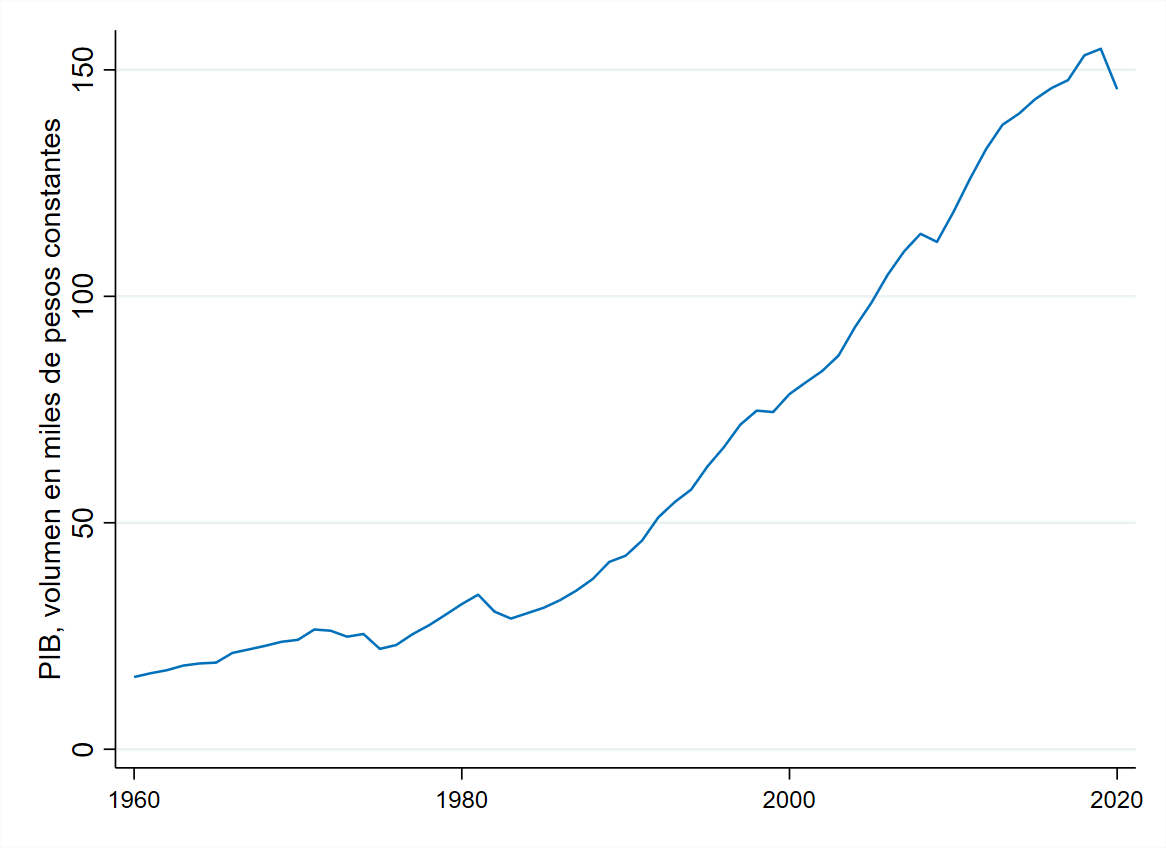
\includegraphics[width=0.6\linewidth]{images/azul.png}
    \end{figure}
    
   
\end{itemize}

\end{frame}
\begin{frame}
\frametitle{El PIB Chileno - Primera Diferencia}

\begin{itemize}
    \item Primera diferencia del PIB

    %                  \begin{figure}
    %     \centering
    %     
\includegraphics[width=0.6\linewidth]{sem14/images/rojo.png}
    % \end{figure}


    \begin{figure}
        \centering
        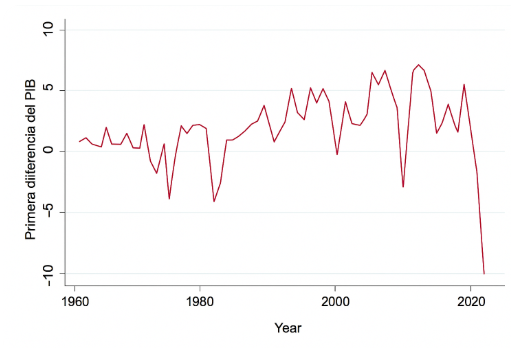
\includegraphics[width=0.7\linewidth]{dif_pib.png}
    \end{figure}
    \item ¿Qu\'e impresi\'on nos da?
\end{itemize}

\end{frame}
\begin{frame}
\frametitle{El PIB Chileno - Ambas Gráficas}

\begin{itemize}
    \item Poniendo ambas gr\'aficas juntas
\end{itemize}

\begin{figure}
    \centering
    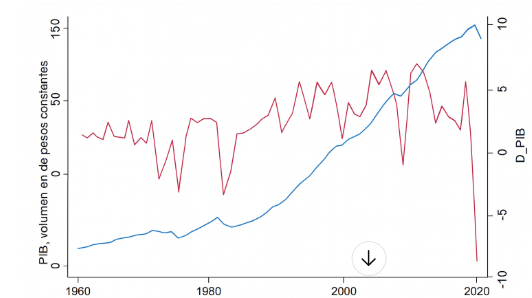
\includegraphics[width=0.7\linewidth]{dif_nivel_pib.png}
\end{figure}

\end{frame}
\begin{frame}
\frametitle{El PIB Chileno - Test de DF}

\begin{itemize}
    \item Realizamos el test de D-F para ver si se trata de una serie integrada de orden 1
    \item Dada nuestra exploraci\'on gr\'afica, corresponder\'ia usar como modelo alternativo el que incluye una tendencia temporal
$$\Delta PIB_t = \alpha + \phi PIB_{t-1} + \delta t +\epsilon_t$$
                     
    \begin{figure}
        \centering
        
\includegraphics[width=0.7\linewidth]{images/pib.png}
    \end{figure}
    
    \item ¿Con qu\'e valor cr\'itico comparamos el estad\'istico t?
\end{itemize}

\end{frame}
\begin{frame}
\frametitle{El PIB Chileno - Test de DF}

\begin{itemize}
    \item Vamos a usar los valores de tabla de DF
    \item $\hat{\phi} = -0.0373029$ y $\hat{\sigma_{\phi}}=0.0228403$ 
    \item Como nuestra muestra es de 60, podemos usar los valores cr\'iticos de la de 50:
    \begin{itemize}
        \item VC al 5\%: -3.50
        \item $| -1.63 | < | -3.50 |$
        \item No rechazo $H_0$
    \end{itemize}
    \item Evidencia a favor de que el PIB chileno tiene una ra\'iz unitaria: no es una serie estacionaria
\end{itemize}

\end{frame}
\begin{frame}[shrink=10]
\frametitle{Conclusiones y Repaso}

\begin{itemize}
    \item Cuando trabajamos con series de tiempo debemos comenzar por ver si las series tienen tendencias temporales: determin\'isticas o estoc\'asticas
    \item Si es determinista, agregamos una tendencia:
    \[
    Y_t = \beta_0 + \beta_1 X_t + \alpha t + u_t
    \]
    \item Interpretaci\'on de $\beta_1$ ahora?
    \item Para saber si tiene una tendencia estoc\'astica (ra\'iz unitaria) procedemos a realizar el test de Dickey-Fuller
    \item Este test tiene valores cr\'iticos espec\'ificos y los mismos dependen del modelo alternativo que nos estemos planteando (con o sin tendencia determin\'istica)
    \item Para determinar el modelo alternativo comenzamos por una exploraci\'on gr\'afica
    \item Si encontramos que la serie tiene una ra\'iz unitaria (no rechazamos $H_0$) vamos a tener que diferenciar la serie y estimar nuestro modelo en diferencias.
\end{itemize}

\end{frame}

% \begin{frame}
% \frametitle{Conclusión}

% \begin{itemize}
%   \item Las series de tiempo muchas veces presentan tendencias:
%   \begin{itemize}
%     \item Determinísticas: cuando la serie varía de forma constante (no aleatoria) con el tiempo.
%     \item Estocásticas: cuando la serie varía de forma variable (aleatoria) con el tiempo.
%   \end{itemize}
%   \item Siempre que haya tendencias, las estimaciones por MCO serán sesgadas: correlaciones espurias (variables omitidas).
%   \item Si la tendencia es determinística: incluimos un regresor que varíe constantemente con el tiempo, por ejemplo, una tendencia lineal.
%   \item Si la tendencia es estocástica: tenemos que usar la primera diferencia de la serie para estimar.
%   \item ¿Cómo sabemos si la serie es integrada de orden 1?
%   \begin{itemize}
%     \newline Se utiliza el test de Dickey-Fuller.
%   \end{itemize}
% \end{itemize}

% \end{frame}


% \begin{frame}
% \frametitle{Procesos Integrados}
% \begin{itemize}
%     \item Muchas series no son estacionarias.
%     \item Una serie es integrada de orden \(d\) si se vuelve estacionaria al diferenciarla \(d\) veces.
%     \item Diferencia de primer orden:
%     \[
%     \nabla Y_t = Y_t - Y_{t-1}
%     \]
%     \item Si \(\nabla^d Y_t\) es estacionaria, entonces \(Y_t \sim I(d)\).
% \end{itemize}
% \end{frame}

% \begin{frame}
% \frametitle{Modelo ARIMA(p,d,q)}
% \begin{itemize}
%     \item Combina:
%     \begin{itemize}
%         \item AR(p): Autorregresivo
%         \item I(d): Diferencias para estacionariedad
%         \item MA(q): Media móvil
%     \end{itemize}
%     \item Notación:
%     \[
%     \phi(L)(1 - L)^d Y_t = \theta(L) \varepsilon_t
%     \]
%     \item \(L\) es el operador de rezago: \(L Y_t = Y_{t-1}\)
% \end{itemize}
% \end{frame}

\end{document}
